% ============================================================
%  Figuras del capítulo 2 del libro digital.
%  Cada tikzpicture sale en su propia página; después se
%  convierten a SVG con:  pdftocairo -svg -f N -l N figuras-cap02.pdf
%  Compilar con pdfLaTeX.
% ============================================================
\documentclass[tikz,border=3pt]{standalone}
\usepackage[T1]{fontenc}
\usepackage{amsmath,amssymb}
\usetikzlibrary{arrows.meta,calc}
\definecolor{turquesaGA}{HTML}{0E7C8C}
\definecolor{turquesaClaro}{HTML}{E2F2F4}
\definecolor{grisT}{HTML}{5F5E5A}
\definecolor{negroP}{HTML}{2B2B2B}
\definecolor{terracota}{HTML}{C1502E}
\definecolor{dorado}{HTML}{B07C10}
\begin{document}

% ---------- 1. Suma de vectores ----------
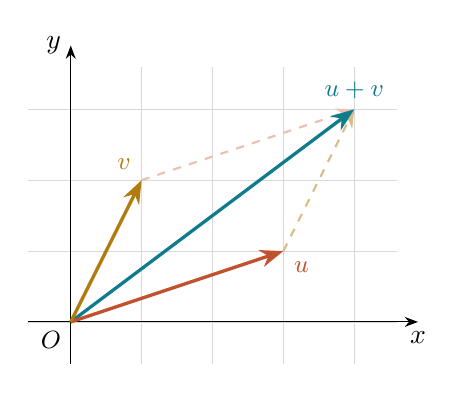
\begin{tikzpicture}[scale=.9,>=Stealth]
  \draw[very thin,color=gray!30] (-0.6,-0.6) grid (4.6,3.6);
  \draw[->] (-0.6,0) -- (4.9,0) node[below]{$x$};
  \draw[->] (0,-0.6) -- (0,3.9) node[left]{$y$};
  \draw[terracota!35,thick,->,dashed] (1,2) -- (4,3);
  \draw[dorado!50,thick,->,dashed] (3,1) -- (4,3);
  \draw[turquesaGA,very thick,->] (0,0) -- (4,3)
    node[above,font=\small]{$u+v$};
  \draw[terracota,very thick,->] (0,0) -- (3,1)
    node[below right,font=\small]{$u$};
  \draw[dorado,very thick,->] (0,0) -- (1,2)
    node[above left,font=\small]{$v$};
  \node[below left,font=\small] at (0,0) {$O$};
\end{tikzpicture}

% ---------- 2. Resta de vectores ----------
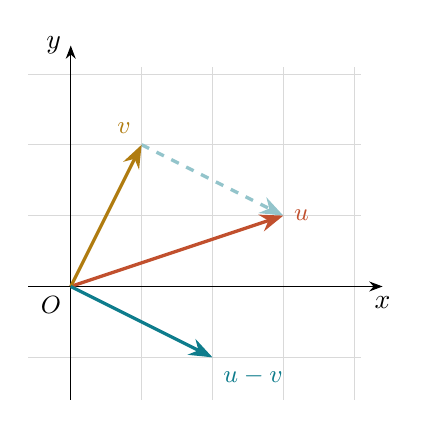
\begin{tikzpicture}[scale=.9,>=Stealth]
  \draw[very thin,color=gray!30] (-0.6,-1.6) grid (4.1,3.1);
  \draw[->] (-0.6,0) -- (4.4,0) node[below]{$x$};
  \draw[->] (0,-1.6) -- (0,3.4) node[left]{$y$};
  \draw[turquesaGA!45,very thick,->,dashed] (1,2) -- (3,1);
  \draw[terracota,very thick,->] (0,0) -- (3,1)
    node[right,font=\small]{$u$};
  \draw[dorado,very thick,->] (0,0) -- (1,2)
    node[above left,font=\small]{$v$};
  \draw[turquesaGA,very thick,->] (0,0) -- (2,-1)
    node[below right,font=\small]{$u-v$};
  \node[below left,font=\small] at (0,0) {$O$};
\end{tikzpicture}

% ---------- 3. Producto por un escalar ----------
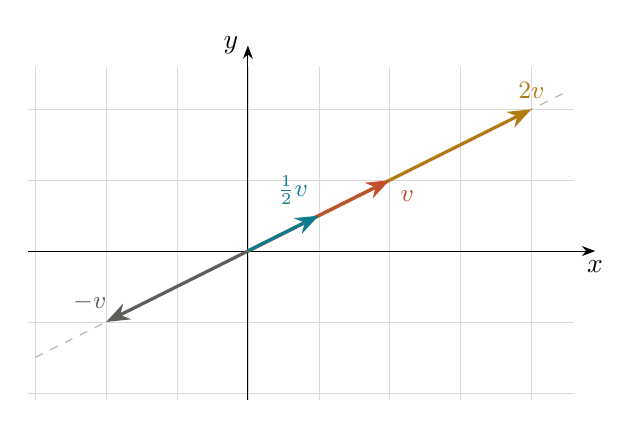
\begin{tikzpicture}[scale=.9,>=Stealth]
  \draw[very thin,color=gray!30] (-3.1,-2.1) grid (4.6,2.6);
  \draw[->] (-3.1,0) -- (4.9,0) node[below]{$x$};
  \draw[->] (0,-2.1) -- (0,2.9) node[left]{$y$};
  \draw[gray!60,dashed] (-3,-1.5) -- (4.5,2.25);
  \draw[dorado,very thick,->] (0,0) -- (4,2)
    node[above,font=\small]{$2v$};
  \draw[terracota,very thick,->] (0,0) -- (2,1)
    node[below right,font=\small]{$v$};
  \draw[turquesaGA,very thick,->] (0,0) -- (1,0.5)
    node[above left,font=\small]{$\tfrac12 v$};
  \draw[grisT,very thick,->] (0,0) -- (-2,-1)
    node[above left,font=\small,xshift=4pt]{$-v$};
\end{tikzpicture}

% ---------- 4. La recta que pasa por el origen ----------
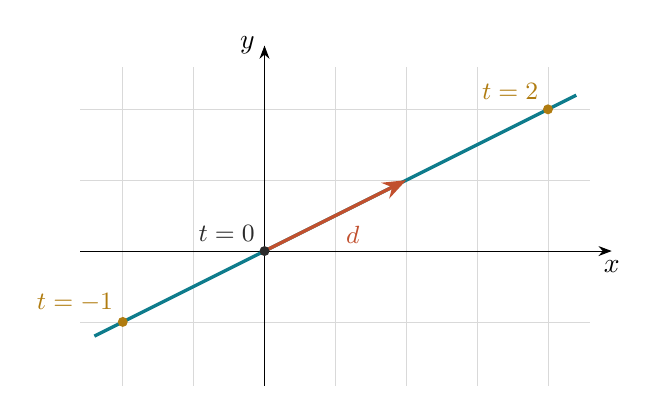
\begin{tikzpicture}[scale=.9,>=Stealth]
  \draw[very thin,color=gray!30] (-2.6,-1.9) grid (4.6,2.6);
  \draw[->] (-2.6,0) -- (4.9,0) node[below]{$x$};
  \draw[->] (0,-1.9) -- (0,2.9) node[left]{$y$};
  \draw[turquesaGA,very thick] (-2.4,-1.2) -- (4.4,2.2);
  \draw[terracota,very thick,->] (0,0) -- (2,1)
    node[midway,below right,font=\small]{$d$};
  \fill[negroP] (0,0) circle(2pt)
    node[above left,font=\small]{$t=0$};
  \fill[dorado] (4,2) circle(2pt)
    node[above left,font=\small]{$t=2$};
  \fill[dorado] (-2,-1) circle(2pt)
    node[above left,font=\small]{$t=-1$};
\end{tikzpicture}

% ---------- 5. La recta trasladada a un punto de paso ----------
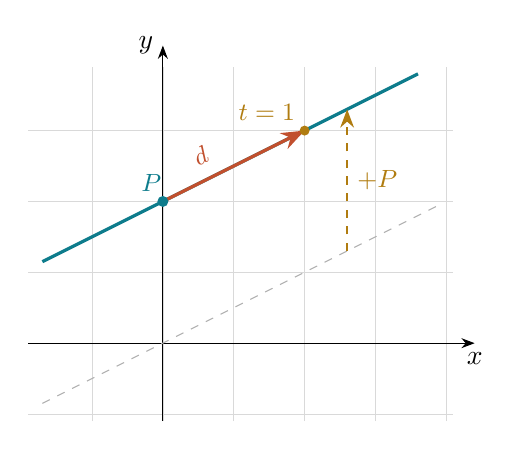
\begin{tikzpicture}[scale=.9,>=Stealth]
  \draw[very thin,color=gray!30] (-1.9,-1.1) grid (4.1,3.9);
  \draw[->] (-1.9,0) -- (4.4,0) node[below]{$x$};
  \draw[->] (0,-1.1) -- (0,4.2) node[left]{$y$};
  \draw[gray!60,dashed] (-1.7,-0.85) -- (3.9,1.95);
  \draw[turquesaGA,very thick] (-1.7,1.15) -- (3.6,3.8);
  \draw[dorado,thick,->,dashed] (2.6,1.3) -- (2.6,3.3)
    node[midway,right,font=\small]{$+P$};
  \draw[terracota,very thick,->] (0,2) -- (2,3)
    node[pos=0.34,above,sloped,font=\small,yshift=1.5pt]{$d$};
  \fill[turquesaGA] (0,2) circle(2.2pt)
    node[above left,font=\small,xshift=3pt]{$P$};
  \fill[dorado] (2,3) circle(2pt)
    node[above left,font=\small]{$t=1$};
\end{tikzpicture}

\end{document}
